\section{QLearning}
\subsection{Princip}
Model-free reinforcement learning algoritmus k zjištění hodnoty akce v konkrétním stavu.
\begin{figure}[h!]
    \centering
    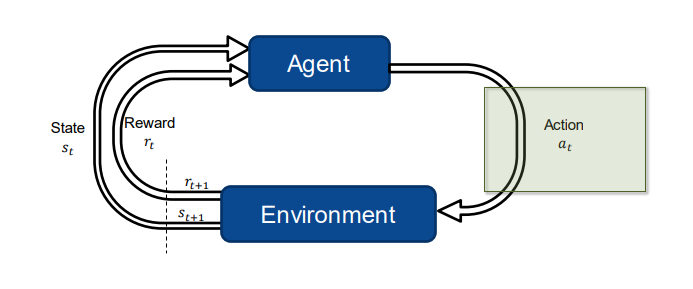
\includegraphics[width=0.5\linewidth]{images/qlearn.png}
    \caption{Q-Learning princip}
    \label{fig:enter-label}
\end{figure}
Základní požadavky:
\begin{itemize}
    \item Prostředí se nemění
    \item Počet stavů a akcí je konečný
    \item Odměny jsou omezené
    \item Rychlost učení se snižuje navštívením párů stav-akce
    \item Exploration metoda garantuje nekonečné navštěvování všech dvojic stav-akce v nekonečné training periodě
\end{itemize}
Nelze vždy zvolit akci s nejvyšší Q hodnotou - Q-funkce je ze začátku neotpimální, je nutno zkoumat možnosti dokud není fce optimální.
Používá se metoda $\epsilon$-hungry, kde se s určitou šancí vykoná náhodná akce, tato pravděpodobnost se postupně snižuje. Agent tedy buď provádí naučenou akci, nebo náhodnou.

\subsection{QLearning vs Sarsa}
Sarsa je on policy algoritmus, používá akci zvolenou současnou policy. Soustředí se na akce které jsou skutečně použity a učí se z následků vlastních rozhodnutí
Q-Learning je off policy, používá greedy approach k naučení se Q-value. SLeduje nejlepší možné akce v každé situaci a učí se z nich.
